% filepath: /home/eswarm/mecanum/Soutenance/6-Resultats/intro.tex

\begin{frame}{Protocole d'expérience}
    \begin{columns}[c]
        \begin{column}{0.5\textwidth}
            La méthode de test est la même pour toutes les expériences :
            \begin{itemize}
                \item 4 robots en formation carrée (Figure \ref{fig:formation}).
                \item Les robots voisins partagent un côté (pas de diagonales).
                \item La trajectoire à suivre est identique pour chaque test (un carré).
            \end{itemize}
        \end{column}
        \begin{column}{0.5\textwidth}
            \begin{figure}
                \centering
                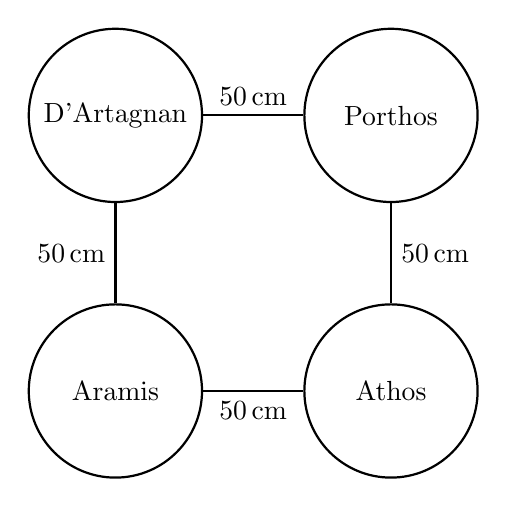
\begin{tikzpicture}[scale=1]
                    \tikzset{robot/.style={circle,draw,minimum size=2.2cm,inner sep=0pt,fill=white,thick,font=\normalsize, text width=2cm, align=center}}
                    \node[robot] (A) at (0,0) {Aramis};
                    \node[robot] (B) at (3.5,0) {Athos};
                    \node[robot] (C) at (3.5,3.5) {Porthos};
                    \node[robot] (D) at (0,3.5) {D'Artagnan};
                    \draw[thick] (A) -- (B) node[midway,below] {50\,cm};
                    \draw[thick] (B) -- (C) node[midway,right] {50\,cm};
                    \draw[thick] (C) -- (D) node[midway,above] {50\,cm};
                    \draw[thick] (D) -- (A) node[midway,left] {50\,cm};
                \end{tikzpicture}
                \caption{Graphe de la formation}
                \label{fig:formation}
            \end{figure}
        \end{column}
    \end{columns}
\end{frame}

\subsection{Démonstration vidéo}
\begin{frame}
    \frametitle{Démonstration vidéo}
    \begin{center}
        \textbf{Exemple vidéo de l'essaim}
        
        \movie[width=8cm,height=6cm,poster,showcontrols]{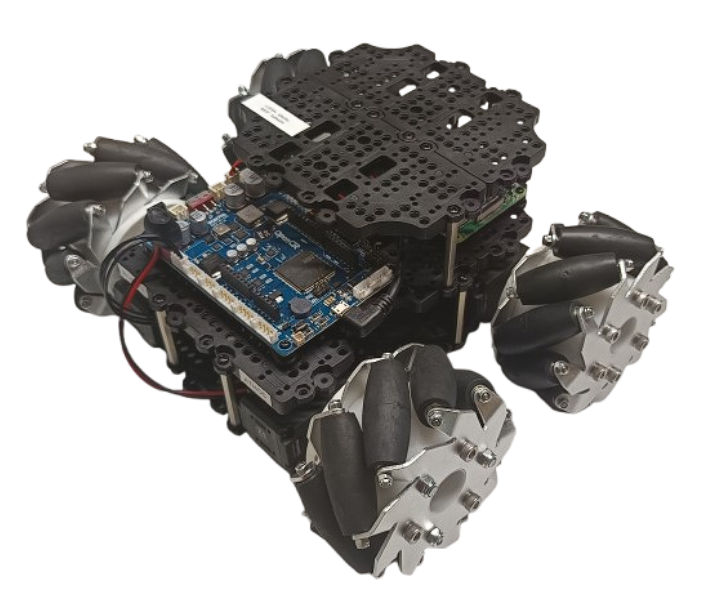
\includegraphics[width=8cm,height=6cm]{video_test/Mecanum.png}}{video_test/montage_turtlebot.mp4}
    \end{center}
\end{frame}
